\documentclass[12pt,preprint]{aastex}
%\usepackage{thumbpdf}
\usepackage{amssymb,float}
\usepackage{psfig,graphicx} 
\usepackage{fullpage,mathtools}
\usepackage{mathrsfs}
\usepackage{natbib}
\usepackage{color}
\usepackage{bm}
\usepackage[title,titletoc,toc]{appendix}
\bibliographystyle{apj}

\addtolength{\oddsidemargin}{-.5in}
\addtolength{\evensidemargin}{-.5in}
\addtolength{\textwidth}{0.5in}

\title{Models and Priors Used in 3D Binary Orbit Simulations}
\author{Kyle Mede}
\date{\today}

\begin{document}

\maketitle

% List contents then list of figures
\tableofcontents


\section{Introduction}

These are the outlines of the functions that act as the models to calculate the orbital elements for either a binary star system or planet orbit.  The equations are the result of combining Kepler's laws, the definitions of the orbital elements and the naturally occurring symmetries and rules of a stable binary system.

There are both Python and C++ versions of these functions/models.  The bulk of the multi-process and file management,  post analysis and plotting of the results is done in Python while the computational stages of the simulation are done in C++ to take advantage of its speed.  A more detailed description of these issues and the simulator will be in another document to be written later.  All three astrometry models described here have been tested and produce the same resulting values/fit to within approximately 10 significant figures, well past the accuracy limits placed on the parameters by their associated 68\% or 95\% errors.

\pagebreak

USEFUL FIGURES REFERENCED IN LATER TEXT, PUT THESE IN A LOGICAL INTRODUCTION OR SOMETHING SOON!!

\begin{figure}[htp]
\begin{center}
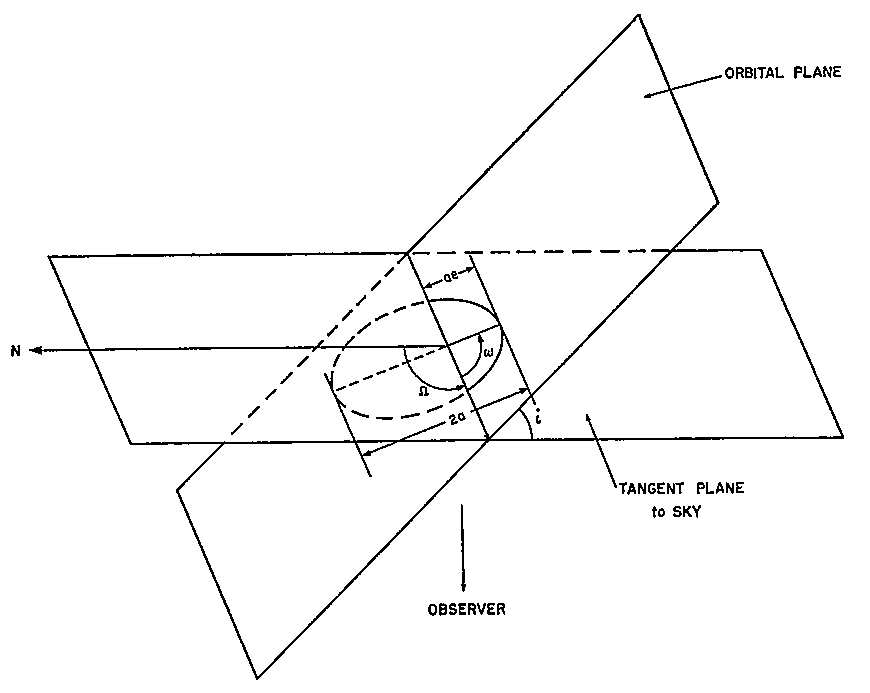
\includegraphics[scale=0.575]{BattenPG8Fig.jpeg}
\caption[Orbital Plane vs Plane of Sky]{ Orbital plane and the tangent plane to the sky  From \citet{batten}. }
\label{fig:OPvsSky}
\end{center}
\end{figure}

\begin{figure}[htp]
\begin{center}
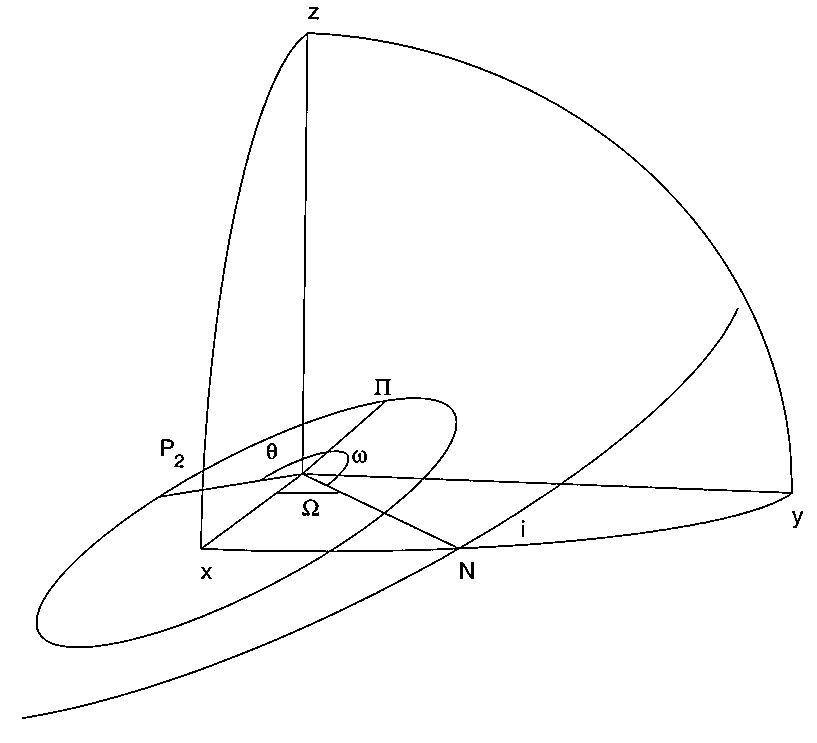
\includegraphics[scale=0.5]{HilditchPG41Fig.jpeg}
\caption[Orbital Elements]{ The relative orbit of a  binary located in three dimensions to show the orbital elements of its orbit.  From \citet{hilditch}. }
\label{fig:orbElements}
\end{center}
\end{figure}

\pagebreak


%----------------------------------------------------------------------------------------------------------------
\section{Simulator Settings}

Here we will go over the large array of settings in the settings file and the possible modes to run the simulator in.

First, lets go through ALL the settings in the "SimSettings" file, as it is where the user is expected to spend the bulk of their time playing around to get things to run the way they want.

{\bf chiSquaredMax}\\
This will set the maximum allowed reduced $\chi^2$ allowed during simple Monte Carlo runs.  During Simulated Annealing it also poses a use to allow the starting parameters to jump to a new set if the chain has yet to find a solution under that value, in this case trial and error are needed but a value around 300 might work at the start and reduced as the parameters are constrained.  That situation can occur if you have a low starting temperature, or the initial parameters are unfortunately in a very bad section of the parameter space.  Thus, the jumping routine helps get out of those ruts and this parameter determines if it is in said rut.

{\bf numSamples}\\
The total number of samples to produce for a single chain.  This is the number of samples for MCMC, Simulated Annealing or Monte Carlo if running in those modes, while the separate Simulated Annealing samples can be controlled with the "numSamples\_SimAnneal" when running in MCMC mode.  Remember that if you use multi-processing, then the true total number of samples will be this number multiplied by how many processes/chains you run.

{\bf numSamplePrints}\\
The number of times a print block will be displayed to the screen of the vital update information for how the simulation is running.  These will occur at sample = numSamples/numSamplePrints intervals during the simulation.

{\bf useMultiProcessing}\\
Turn on multi-processing?  If set to true, then there will be multiple chains started.  The current code will start \# chains = total number of virtual cores available - 1, leaving one core free to make sure the computer OS still runs smooth. ie. on an computer with a 8 virtual cores (4 cores with 2 threads each), 7 cores will run a chain at 100\% capacity and 1 will be left remaining to do anything else.  If the user wishes, they can go into the code and change the single line that controls the number of cores used to suite their needs.  Please note that each core will be running at $\sim$100\%, and thus create a lot of heat.  So, make sure you have a sufficiently capable cooler to avoid CPU failure.

{\bf silent}\\
There are two levels of extra information printing above that of the print block controlled with "numSamplePrints", or any error prints due to problems.  The higher level one is "silent", with some extra prints that will occur for each sample and is useful for some debugging.


{\bf verbose}\\
This is the second level of debug print messages.  It will basically trigger the simulator to give you a high level of verbosity to its step by step process, including for all the pre-simulation file checking and such.

{\bf settings\_and\_InputDataDir}\\
The full path to where your input settings directory is.  

{\bf SystemDataFilename}\\
Name of the file for the system data.  Just leaving this to the standard "SystemData.txt" and using the prepending approach has proved the most useful for me.

{\bf DIdataFilename}\\
Name of the file for the astrometry data.  Just leaving this to the standard "DIData.dat" and using the prepending approach has proved the most useful for me.

{\bf RVdataFilename}\\
Name of the file for the radial velocity data.  Just leaving this to the standard "RVData.dat" and using the prepending approach has proved the most useful for me.

{\bf outputData\_dir}\\
The full path to where the output data will be written.  The simulator will create a sub-directory in here based on the "outputData\_filenameRoot" setting.

{\bf outputData\_filenameRoot}\\
The root file name to use for the output folder and will also be used as part of the titles of the output plots and such.

{\bf RVonly}\\
Only perform fitting to the radial velocity data?  Set both this and "DIonly" to false to use 3D fitting.

{\bf DIonly}\\
Only perform fitting to the astrometry data?  Set both this and "RVonly" to false to use 3D fitting.

{\bf simAnneal}\\
Run only Simulated Annealing?  This is a good way to make sure that the Simulated Annealing stage is running well and finding a suitable starting place for the following MCMC simulations.

{\bf loopedMCMC}\\
This might be still broken when you download SMODT, but it is designed to run bootstrap type simulations on a special version of the input data, maybe only the RV data.  There are functions to produce a set of the RV data with re-arranged errors.  If many of these data sets are created, this version of the simulator would run on each data set and give different final solutions for each, that can all be plotted together to give an idea of the output solution set's range.  It was suggested by some and thus implemented, but later given up on.

{\bf makePosteriorsPlot}\\
Make plots of the posterior distributions?  These will be histograms of the output values from Monte Carlo or MCMC, but not possible with Simulated Annealing by definition of how it runs.

{\bf makeOrbitPlots}\\
Make plots of the orbits, both astrometry and radial velocity if requested with "RVonly" and "DIonly", with the data also represented.  Tweaks to these plots can be made in the Python "plotToolbox.py" file if the user wishes.

{\bf makeSimAnnealProgPlots}\\
Make progress plots of the Simulated Annealing run.  This is a time series showing the values of all the varying parameters as a function of sample number.  It is useful for seeing how the simulation converges to the final parameters.

{\bf startTemp}\\
Starting temperature for the Simulated Annealing runs.  Anything between 50-1000 could work, but it depends on how long you want to run that stage of the simulation for and how well constrained the parameters are.

{\bf delChainsAfter}\\
Delete the output data files for each chain after the simulation is complete?  This is a good way to save you from filling up your disk space when running many successive simulations.  Remember that long simulations (over say 1e8) an cause large output data files on the order of hundreds of Gigabites.

{\bf delCombinedDataAfter}\\
Delete the combined data file after simulation completes?  After processing anything needed for the individual chains, they are combined to make a final single output data file (in the cases of MCMC and Monte Carlo only).  Again, deleting these after can help save space.

{\bf TcStepping}\\
The simulator calculates the Time of Last Periapsis (To) from other parameters and the Time of Center Transit (Tc), or vice versa.  In the cases of very low eccentricities (under 0.3) it is recommended to step through the parameter space in Tc to help avoid biasing towards higher eccentric orbits.  Thus, set this to true to do just that, or set it to false to calculate Tc from the varying To values.

{\bf CopyToDrobox}\\
If you like, you can define the location of a DropBox directory, or another directory, you wish the smaller files produced by the simulator (plots, and maybe the log files) to be copied to at the end of the simulation.  This is useful for showing collaborators recent results, or for you to see results on your home computer when running it on your work desktop.

{\bf CalcBurnIn}\\
The burn in is the stage of the MCMC where the chain is "forgetting" its starting point.  This is hopefully handled during the final sigma tunning at the end of the Simulated Annealing stage, but if it is a much larger value, then you should consider deleting the samples from the MCMC chains to remove any bias caused by the starting location.

{\bf calcCorrLengths}\\
Another way to look at the progress of an MCMC chain is its correlation length.  This will tell you how well the chain really explores the parameter space.

{\bf numSamples\_SimAnneal}\\
When running MCMC mode, this will set the number of samples for the Simulated Annealing stage.

{\bf makeMCMCprogPlots}\\
Make progress plots of the MCMC chains.  Just like the earlier setting for the Simulated Annealing chains, this can give you another visual way to investigate how the MCMC chains are exploring the parameter space.  As MCMC is statistically designed to explore the space efficiently, this is commonly useless, but could pose useful to some users.

{\bf CalcGelmanRubin}\\
The Gelman Rubin statistic (R) gives an indication on the simulations convergence to the final posterior distribution.  R values of 1.0 indicate a perfect convergence, while values much higher indicate the simulation needs to be ran longer.  Typically R $\leq1.1$ is considered the criterion for convergence.

{\bf numTimesCalcGR}\\
How often should the R values be calculate?  This calculation is very heavy, so a smaller number is good, but remember you also want to know how the simulation is progressing as well.  A happy middle would be $\sim$ 100.

{\bf simulate\_StarStar }\\
Simulate a Star-Star system?  ie. a binary.

{\bf simulate\_StarPlanet}\\
Simulate a Star-Planet system?

{\bf longAN\_degMIN}\\
Minimum value for the Longitude of the Ascending node parameter.
Zero for the MIN and MAX values indicate to not let it vary.  Or you could set it to very tight values around a fixed value if you like.

{\bf longAN\_degMAX}\\
Maximum value for the Longitude of the Ascending node parameter.
Zero for the MIN and MAX values indicate to not let it vary.  Or you could set it to very tight values around a fixed value if you like.

{\bf eMIN}\\
Minimum value for the Eccentricity parameter.
Zero for the MIN and MAX values indicate to not let it vary.  Or you could set it to very tight values around a fixed value if you like.

{\bf eMAX}\\
Maximum value for the Eccentricity parameter.
Zero for the MIN and MAX values indicate to not let it vary.  Or you could set it to very tight values around a fixed value if you like.

{\bf periodMIN}\\
Minimum value for the Period parameter.
Zero for the MIN and MAX values indicate to not let it vary.  Or you could set it to very tight values around a fixed value if you like.

{\bf periodMAX}\\
Maximum value for the Period parameter.
Zero for the MIN and MAX values indicate to not let it vary.  Or you could set it to very tight values around a fixed value if you like.

{\bf a\_totalMIN}\\
Minimum value for the total Semi-Major Axis parameter.  The sum of both body's semi-major axes.
Zero for the MIN and MAX values indicate to not let it vary.  Or you could set it to very tight values around a fixed value if you like.  The masses of the stars, or planet, will be used to calculate their individual semi-major axes when performing radial velocity fitting.  The a\_total value can also be calculated from Kepler's third law, using the period and masses, so set MIN and MAX values to trigger this. 

{\bf a\_totalMAX}\\
Maximum value for the total Semi-Major Axis parameter.  The sum of both body's semi-major axes.
Zero for the MIN and MAX values indicate to not let it vary.  Or you could set it to very tight values around a fixed value if you like.  The masses of the stars, or planet, will be used to calculate their individual semi-major axes when performing radial velocity fitting.  The a\_total value can also be calculated from Kepler's third law, using the period and masses, so set MIN and MAX values to trigger this. 

{\bf inclination\_degMIN}\\
Minimum value for the Inclination parameter.
Zero for the MIN and MAX values indicate to not let it vary.  Or you could set it to very tight values around a fixed value if you like.

{\bf inclination\_degMAX}\\
Maximum value for the Inclination parameter.
Zero for the MIN and MAX values indicate to not let it vary.  Or you could set it to very tight values around a fixed value if you like.

{\bf argPeri\_degMIN}\\
Minimum value for the Argument of Periapsis parameter.
Zero for the MIN and MAX values indicate to not let it vary.  Or you could set it to very tight values around a fixed value if you like.

{\bf argPeri\_degMAX}\\
Maximum value for the Argument of Periapsis parameter.
Zero for the MIN and MAX values indicate to not let it vary.  Or you could set it to very tight values around a fixed value if you like.

{\bf T\_Min}\\
Minimum value for the Time of Last of Periapsis parameter, OR, the Time of Center Transit if TcStepping=True.
Zero for the MIN and MAX values indicate to not let it vary and instead take it as a fixed value from the SystemData.txt file.  -1 indicates to use [earliestsEpoch-period,earliestEpoch], with earliestEpoch being the earliest observation in the data between the astrometry and RV data files.  Or you could set it to very tight values around a fixed value if you like.

{\bf T\_Max}\\
Maximum value for the Time of Last of Periapsis parameter, OR, the Time of Center Transit if TcStepping=True.
Zero for the MIN and MAX values indicate to not let it vary and instead take it as a fixed value from the SystemData.txt file.  -1 indicates to use [earliestsEpoch-period,earliestEpoch], with earliestEpoch being the earliest observation in the data between the astrometry and RV data files.  Or you could set it to very tight values around a fixed value if you like.

{\bf K\_MIN}\\
Minimum value for the Radial Velocity Semi-Major Amplitude parameter.  It will only vary if DIonly==false and inclination\_degMAX==0.  Else, it will be calculated from other values.
Zero for the MIN and MAX values indicate to not let it vary.  Or you could set it to very tight values around a fixed value if you like.  This value can be calculated from the masses, inclination and semi-major axes as well, so set the MIN and MAX values to zero to do calculate it that way instead.

{\bf K\_MAX}\\
Maximum value for the Radial Velocity Semi-Major Amplitude parameter.  It will only vary if DIonly==false and inclination\_degMAX==0.  Else, it will be calculated from other values.
Zero for the MIN and MAX values indicate to not let it vary.  Or you could set it to very tight values around a fixed value if you like.  This value can be calculated from the masses, inclination and semi-major axes as well, so set the MIN and MAX values to zero to do calculate it that way instead.

{\bf RVoffsetMINs}\\
Minimum value for the Radial Velocity Offset parameter.  This will be a list, with one value for each RV data set provided.
Zero for the MIN and MAX values indicate to not let it vary.  Or you could set it to very tight values around a fixed value if you like.

{\bf RVoffsetMAXs}\\
Maximum value for the Radial Velocity Offset parameter.  This will be a list, with one value for each RV data set provided.
Zero for the MIN and MAX values indicate to not let it vary.  Or you could set it to very tight values around a fixed value if you like.


%----------------------------------------------------------------------------------------------------------------

\section{Priors}\label{sec:priors}

In order to include previously determined information about the distribution some of the parameters tend to be for binary systems, sometimes non-uniform priors were used in the Metropolis-Hastings equation for the MCMC simulations.

As found by \citet{duquennoy1991}, for systems with periods$\geq$1000 days, a function of f({\it e})=2{\it e} can be fit to their distribution, else no strong trend was seen.  Thus, we adopt this result and use the normalized prior probability in Equation (\ref{eq:eProb1000}) for cases when the period is likely well over 1000days.  Although, for those systems with close-in planets, the parametrizations $\sqrt{{\it e}}$ $\cos(\omega$) and $\sqrt{{\it e}}$ $\sin(\omega$) are used to allow for more efficient sampling and convergence when the eccentricity is very low ($\le$0.1), following the suggestion in \citet{albrecht2012}. This new parametrization result in a flat prior for {\it e} and $\omega$.
\begin{equation}\label{eq:eProb1000}
P_n(e) =  2e
\end{equation}

%\begin{equation}\label{eq:eProb}
%P_n(e) =  \frac{1}{e_{max}-e_{min}}
%\end{equation}
 
To take account for the random possible orbital orientations, a prior proportional to sin(i) is used, (\ref{eq:iProb}).

\begin{equation}\label{eq:iProb}
P_n(i) =  \frac{\sin(i)}{\cos(i_{min})-\cos(i_{max})}
\end{equation}

For situations where the data of the orbit is sparsely sampled, such as in the case systems with periods over a month, one must be careful to avoid aliasing that can lead to a multitude of orbital period solutions.  This effect is thoroughly discussed in \citet{gregory2005}, and the suggestion of using a Jeffreys prior was described as the adequate solution to this problem, (\ref{eq:pProb}).

\begin{equation}\label{eq:pProb}
P_n(P) =  \frac{1}{P ln(\frac{P_{max}}{P_{min}})}
\end{equation}

Assuming the data is Gaussian distributed, the rejection function of the Metropolis-Hastings algorithm reduces to (\ref{eq:metHastingsReduced}) once these normalized priors for orbits over 1000days are taken into account.  For those cases where the orbit is well under 1000days, or if $\sqrt{{\it e}}$ $\cos(\omega$) and $\sqrt{{\it e}}$ $\sin(\omega$) are used, the ratio of the eccentricities in (\ref{eq:metHastingsReduced}) simply becomes 1.

\begin{equation}\label{eq:metHastingsReduced}
r(X_t,X_p) = max\bigg\{1, \frac{P_t}{P_p}\frac{e_p}{e_t}\frac{\sin(i_p)}{\sin(i_t)}e^{\frac{(\chi^2_t - \chi^2_p)}{2}} \bigg\}
\end{equation}
where, $\chi^2$ is the chi squared fit to the data given by (\ref{eq:chiSquared}).

\begin{equation}\label{eq:chiSquared}
{\chi}^{2} \equiv  \sum_{i=1}^{i=E} \frac{(model_i - observed_i)^{2}}{\sigma^{2}_i}
\end{equation}

%\clearpage

\pagebreak

%----------------------------------------------------------------------------------------------------------------------------------

\section{Models}

\subsection{True Anomaly Calculator}\label{sec:TAcalc}
The True Anomaly Calculator is used for both models as it is more general.
%\subsubsection{Inputs}

\begin{table}[h]
\centering
\caption{ Inputs to the True Anomaly Calculator.}
\begin{tabular}{c c c}
\hline\hline
Parameter & Description & Typical Range \\
\hline
t* & epoch of observation/image [julian date] & n/a\\
e & eccentricity of orbits [unitless] & [0.001,0.999]\\
T & Last Periapsis Epoch/time [julian date] & [t-period,t]\\
$T_c$* & Last Transit Center Epoch/time [julian date] & [t-period,t]\\
period & period of orbits [yrs] & [1.0,100.0]\\
verbose & Send prints to screen? [True/False](Default = False) & n/a\\
\hline
\end{tabular}
\\
 * = Normally measured/known (ie. not random numbers).
\end{table}

%\subsubsection{Outputs}

\begin{table}[h]
\centering
\caption{ Outputs of the True Anomaly Calculator.}
\begin{tabular}{c c}
\hline\hline
Parameter & Description \\
\hline
n** & Mean Motion [rad/yr] \\
M** & Mean Anomaly [$^{\circ}$]\\
E & Eccentric Anomaly [$^{\circ}$]\\
$\theta$ & True Anomaly [$^{\circ}$]\\
\hline
\end{tabular}
\\
 ** = Not currently returned, but easily could be if needed.
\end{table}
\pagebreak

First calculate the Mean Motion from the provided period:
\begin{equation}\label{eq:4.1.1}
n = \frac{2\pi}{period} 
\end{equation}

Use the Mean Motion (n), time of current epoch (t) and time of last periapsis (T) to get the Mean Anomaly (M):
\begin{equation}\label{eq:4.1.2}
M = n \bigg( \frac{(t-T)}{365.25} \bigg)
\end{equation}

The relation between the Eccentric Anomaly (E) and the Mean Anomaly is given by Kepler's equation, and is a transcendental equation that must be solved using numerical methods.
\begin{equation}\label{eq:4.1.3}
M = E - {\it e}\times\sin(E)
\end{equation}
In order to obtain the solution for E the fastest using the Newton's loop and (\ref{eq:4.1.4}), the closest guess of E should be used as the initial value of E$^{\prime}$.  This also helps to avoid ending up with one of the wrong solutions in cases where there are multiple crossings of the two functions that make up Equation (\ref{eq:4.1.3}).  A suggested initial guess that we found to work well is given by (\ref{eq:4.1.3.5}), found by \citep{Argyle}.

\begin{equation}\label{eq:4.1.3.5}
E_0 = M+{\it e}\sin(M) + \frac{e^2}{2M}sin(2M)
\end{equation}

Newton's method to calculate E is then given by repeatedly calculating (\ref{eq:4.1.4}) in a loop:
  
\begin{equation}\label{eq:4.1.4}
E^{\prime \prime} = E^{\prime} - \frac{[E^{\prime} - {\it e} \times \sin(E^{\prime}) - M]}{[1.0 - {\it e} \times \cos(E^{\prime})]}
\end{equation}
The loop completes when {\it E$^{\prime \prime}$} and {\it E$^{\prime}$} are the same to 10 decimal places.  It is also checked to ensure the resulting value for {\it E} satisfies the original Equation (\ref{eq:4.1.3}) with the same precision.  The maximum value of {\it e}possible was found to be ~0.98, as rounding issues caused a division by zero above this.\\

Using the resultant {\it E} the True Anomaly ($\theta$) can be calculated following:
\begin{subequations}
\begin{align}
\label{eq:4.1.5a}
\theta^{\prime}& = \cos^{-1} \bigg( \frac{[\cos(E) - e]}{[1.0 -{\it e}\times \cos(E)]} \bigg)\\
\label{eq:4.1.5b}
\theta& = \left\{ \begin{array}{l l} \theta^{\prime}& \quad \text{ if E $\leq$ 180$^{\circ}$}\\ 360^{\circ}  - \theta^{\prime}& \quad \text{ if E $>$ 180$^{\circ}$} \end{array}\right.
\end{align}
\end{subequations}
Equation (\ref{eq:4.1.5a}) has the unfortunate attribute that as the Eccentric Anomaly grows over 180$^{\circ}$, the resulting value for the True Anomaly goes down, rather than up as should happen.  This problem is rectified by applying the conditional statements of (\ref{eq:4.1.5b}).\\  

The pictorial representation of these three anomalies is summarized in Figure \ref{fig:Anomalies}.

\begin{figure}[ht]
\begin{center}
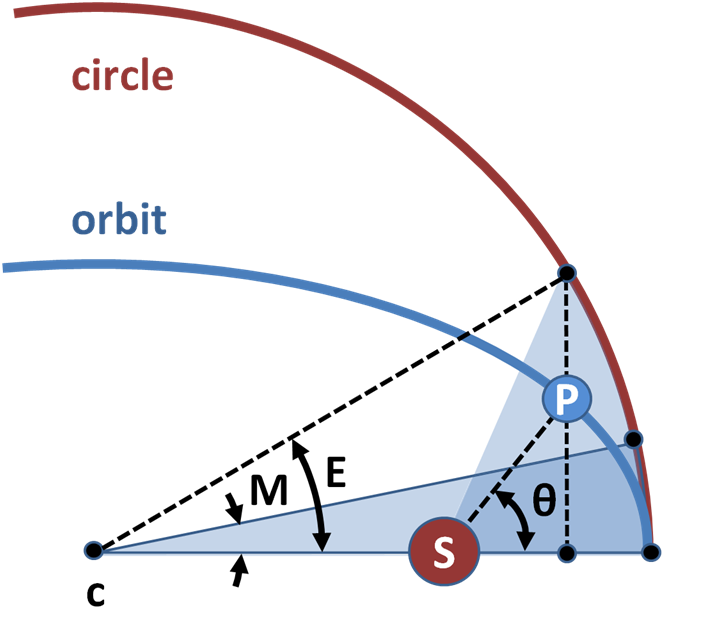
\includegraphics[scale=0.4]{Anomalies-MOD.png}
\caption[Diagram of Anomalies]{A diagram to compare the Eccentric, Mean and True anomalies of an orbiting planet.  The planet is marked as P, the central is S, and the center of the ellipse is C in this plot. }
\label{fig:Anomalies}
\end{center}
\end{figure}
%----------------------------------------------------------------------------------------------------------------------------------
\subsection{Converting between $T_o$ and $T_{ij}$}\label{sec:ToTcCalculator}

Used by the Radial Velocity model, not needed by the Astrometry model and is thus set to zero for those calculations.

In order to avoid biasing against circular solutions, one approach is to step through the parameter space using the Time of Inferior Conjunction ($T_{ij}$), instead of the Time of Periapsis ($T_o$).  From the Earth's prospective, $T_{ij}$ is when the companion object is located between the Earth and the primary (shown as {\color{green}$T_{ij}$} in Figure \ref{fig:ToTcDiagram}), and $T_o$ is when the companion crosses the plane of the sky moving away from the Earth, \citep{heintz}.  In the radial velocity method, at $T_{ij}$ the motion of the planet will be completely parallel to the plane of the sky, with no component along the line of sight to the Earth, resulting in a measured radial velocity of zero.  By understanding these two definitions, it is possible to calculate one from the other if the values for the eccentricity, {\it e}, and argument of periapsis, $\omega$, are known.

First, considering the plane of the sky is perpendicular to the line of sight (see Figures \ref{fig:orbElements} \& \ref{fig:ToTcDiagram}), it can be understood that the True Anomaly ($\theta_s$) of the companion at the Time of Inferior Conjunction will equal 90$^{\circ}$.  Then:

\begin{equation}\label{eq:one}
\theta_s = 90^{\circ}-\omega
\end{equation}

When the companion passes in front of the primary directly along the line-of-site, this location is referred to as the Time of Center Transit ($T_c$).  Although, in many cases the inclination of the system is not in the $90^{\circ}$+/-$10^{\circ}$ rough ranged needed, and no transit will be seen from Earth.

The Eccentric Anomaly of the companion can then be calculated from:

\begin{equation}
E_s = 2.0*\tan^{-1} \bigg( \sqrt{\frac{1.0-e}{1.0+e}} \frac{\sin(\frac{\theta_s}{2.0})}{\cos(\frac{\theta_s}{2.0})} \bigg)
\end{equation}
this equation is a manipulated version of that found in many texts, such as \citet{heintz}, seen below.

\begin{equation}
\tan\bigg( \frac{\theta_s}{2.0}  \bigg) = \sqrt{\frac{1.0+e}{1.0-e}} \tan\bigg( \frac{E_s}{2.0} \bigg)
\end{equation}

The Kepler's Equation, where $M_s$ is the Mean Anomaly of the secondary, (\citet{heintz} \& \citet{hilditch}), is given by:

\begin{equation}
M_s = E_s-e\times \sin(E_s)  
\end{equation}

Knowing the relations for the Mean Motion n:

\begin{subequations}
\begin{align}
n &= \frac{2\pi}{P}\\
n &=\frac{M_s}{t-T_o}=\frac{M_{ij}-M_{o}}{T_{ij}-T_o} 
\end{align}
\end{subequations}
where {\it t} is the epoch of observation and P is the orbital period.
We can then apply these to get the following equation assuming $M_{o}$ is zero.

\begin{equation}\label{eq:five}
\Delta t =t = \frac{M_{ij}P}{2\pi}
\end{equation}

%The value of $\Delta$t is forced to be inside one positive period by adding the period to it if (\ref{eq:5}) results in a negative value.

From this we can calculate either the Time of Inferior Conjunction, or Time of Periapsis knowing the other using:
\begin{subequations}
\begin{align}
T_{ij} &= T_{o}+\Delta t\\
T_o &= T_{ij}-\Delta t
\end{align}
\end{subequations}

%Extra non-necessary equations for my work, but I am writing them up for completion of the equations provided in the email.

%Finally a ratio of location in the orbit compared to periastron is calculated, this can also be thought of as a version of the orbital phase:
%\begin{equation}
%d_{min_s} = \frac{\Delta t}{P}
%\end{equation}

Knowing the primary object is just 180$^{\circ}$ out of phase with the companion, these equations can be used for the primary replacing $\theta_p$ for $\theta_s$ in Equation (\ref{eq:one}):
\begin{equation}
\theta_p = \frac{\pi}{2.0}-\omega+\pi
\end{equation}


\begin{figure}[htp]
\begin{center}
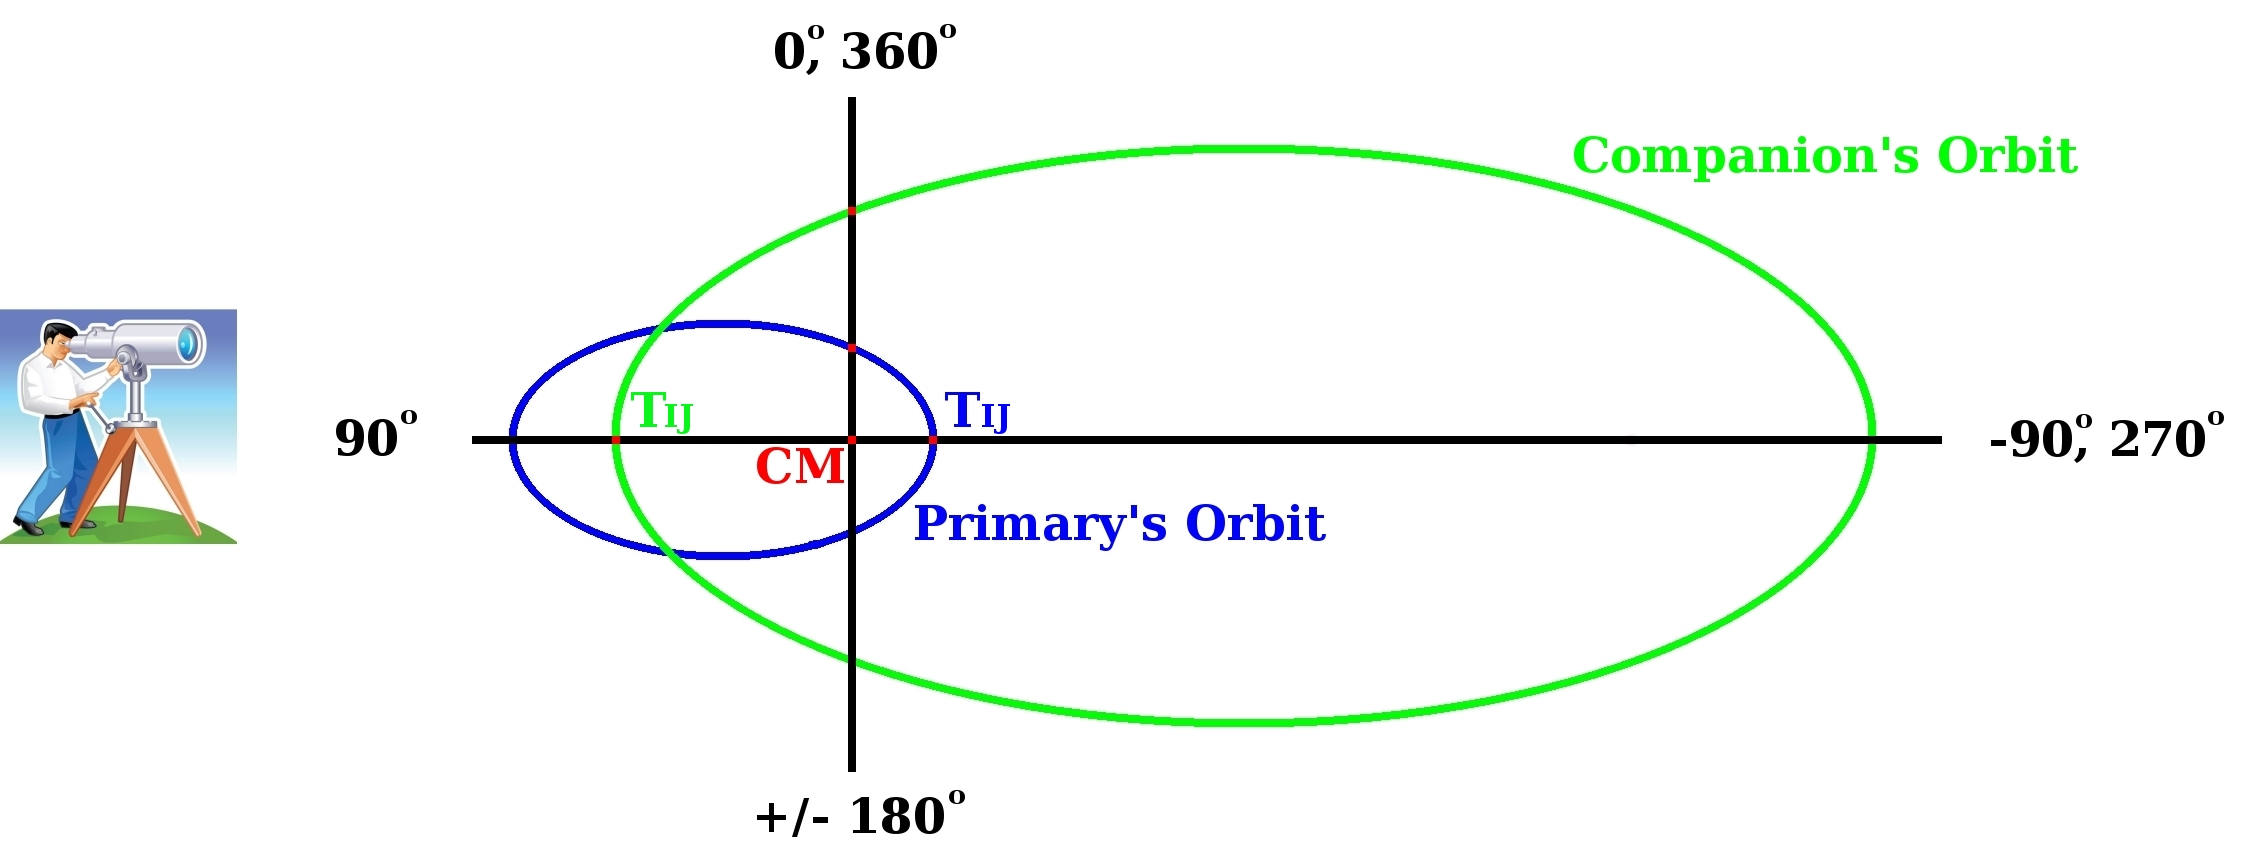
\includegraphics[scale=0.31]{TcToEllipses2-withTelescope4.jpeg}
\caption[Binary Inferior Conjunction Diagram]{A diagram showing the location of the Inferior Conjunction locations ({\color{green}$T_{ij}$} \& {\color{blue}$T_{ij}$}) of two objects in a binary system, orbiting the center of mass ({\color{red}CM}).}
\label{fig:ToTcDiagram}
\end{center}
\end{figure}

To take into account that $T_{ij}$ can occur before or after $T_{o}$ in a given system, the following conditionals are applied to get the correct value for $\Delta t$ produced by Equation (\ref{eq:five}):

\begin{equation}\label{eq:ToTcCorrections1a}
\Delta t = \left\{ \begin{array}{l l} \Delta t-P& \quad \text{ $\omega$ in [ 90$^{\circ}$,360$^{\circ}$], (T$_o$ $>$ T$_{ij}$)}\\  \Delta t& \quad \text{ $\omega$ in [-180$^{\circ}$,90$^{\circ}$], (T$_o$ $<$ T$_{ij}$)} \end{array} \right.
\end{equation}

these simplify to:
\begin{equation}\label{eq:ToTcCorrections1b}
\Delta t = \left\{ \begin{array}{l l} \Delta t-P& \quad \text{ $\omega$ $>$ 90$^{\circ}$, (T$_o$ $>$ T$_{ij}$)}\\  \Delta t& \quad \text{ otherwise , (T$_o$ $<$ T$_{ij}$)} \end{array} \right.
\end{equation}

When considering the values for the primary object, these conditionals become:

\begin{equation}\label{eq:ToTcCorrections2a}
\Delta t = \left\{ \begin{array}{l l} \Delta t-P& \quad \text{ $\omega$ in [-180$^{\circ}$,270$^{\circ}$], (T$_o$ $>$ T$_{ij}$)}\\  \Delta t& \quad \text{ $\omega$ in [ 270$^{\circ}$,360$^{\circ}$], (T$_o$ $<$ T$_{ij}$)} \end{array} \right.
\end{equation}

simplifying to:
\begin{equation}\label{eq:ToTcCorrections2b}
\Delta t = \left\{ \begin{array}{l l} \Delta t-P& \quad \text{ $\omega$ $>$ 270$^{\circ}$, (T$_o$ $>$ T$_{ij}$)}\\  \Delta t& \quad \text{ otherwise , (T$_o$ $<$ T$_{ij}$)} \end{array} \right.
\end{equation}

Therefore, with these equations, one only needs to step through the parameter space along one of them and calculate the other from it along with {\it e}, P and $\omega$.

%-------------------------------------------------------------------------------------------------------------
\subsection{Differences Between Investigating Stellar or Planetary Companion}\label{sec:omegaIssues}

The key difference when investigating a planetary compared to that of a stellar companion is the values of {\it a} and $\omega$ used in the astrometry model.  As discussed in \citet{Shulze-Hartung} and \citet{wright2009}, when the companion is a planet, the values of for the star are used, ie $a_1$ and $\omega_1$.  This is because the method was originally developed to find the orbit of the primary about the system's center of mass as the secondary was not seen.  More recently though, in most cases the companion is seen and the astrometric values are for the location of the secondary relative to the primary instead of the center of mass.  In these cases the apparent orbit is for the combined system and the values input into the astrometric model are $a_1+a_2$ and $\omega_2+\pi$, using the convention $\omega_1$ = $\omega_2+\pi$.

One must be careful to take this into account when doing 3D simulations, to ensure that $\omega_2+\pi$ is passed into the astrometry model and simply $\omega_2$ is used in the radial velocity one.

\pagebreak
%----------------------------------------------------------------------------------------------------------
\subsection{Direct Imaging (Astrometry) Model}\label{sec:DI-OrbModels}
There are two versions of this model, the one used by C++ for the simulation, and the one used by Python in the post processing and plotting.  Both have been checked to ensure the produce the same results for a given set of inputs.  They were chosen to be optimized for each purpose.
%--------------------------------------------------------------------------------------------------------------------------------------

\subsubsection{Full Equations Approach}

This is the approach used in the Python post-processing.

One method by which to form a model for the apparent ellipse for the orbit of a companion measured with astrometry is to develop them from base equations.  Thus, the equations here are the result of combining Kepler's laws, the definitions of the orbital elements and the naturally occurring symmetries and rules of a stable binary system.\\

%\subsubsection{Inputs}
\begin{table}[h]
\centering
\caption{ Inputs to the Astrometry Model.}
\begin{tabular}{c c c}
\hline\hline
Parameter & Description & Typical Range \\
\hline
t* & epoch of observation/image [Julian date] & n/a\\
Sys$\_$Dist* & measured system distance from Earth [PC] &  [0.01,50.0]\\
$\rho$* & Measured Separation Angle ["] & [0.01,10.0]\\
$\Delta\rho$* & Error in Measured Separation Angle ["] & [0.01,10.0]\\
$\phi$*  & Measured Position Angle  [$^{\circ}$] & [0,360]\\
$\Delta\phi$*  & Error in Measured Position Angle  [$^{\circ}$] & [0,360]\\
{\it i} & inclination [$^{\circ}$] & [0,180]\\
$\Omega$ & Longitude of Ascending Node [$^{\circ}$] & [0,360]\\
$\omega$ & Argument of Periapsis [$^{\circ}$] & [0,360]\\
e & eccentricity of orbits [unitless] & [0.001,0.999]\\
T & Last Periapsis Epoch/time [julian date] & [t-period,t]\\
period & period of orbits [yrs] & [1.0,100.0]\\
a*** & Total Semi-major axis [AU]  & [0.1,200] \\
Mass1*** & Mass of primary star [M$_{\sun}$] & [0.001,10] \\
Mass2*** & Mass of companion [M$_{\sun}$] & [0.001, Mass1] \\
verbose & Send prints to screen? [True/False](Default = False) & n/a\\
\hline
\end{tabular}
\\
 * = Normally measured/known (ie. not random numbers).\\
 *** = Optional.
\end{table}

%\subsubsection{Outputs}

\begin{table}[h]
\centering
\caption{ Outputs of the Astrometry Model.}
\begin{tabular}{c c}
\hline\hline
Parameter & Description \\
\hline
$\chi^{2}_{\nu}$ & Reduced Chi Squared \\
a & Total Semi-major axis [AU]  \\
\hline
\end{tabular}
\end{table}

\pagebreak

First the True Anomaly calculator (\ref{sec:TAcalc}) is used to calculate E and $\theta$, the Eccentric and True Anomalies respectively.

The True Anomaly can then be used to find the Separation Distance in the orbital plane ($R^{\prime}$), split that into its X and Y components (WRT Line of Nodes) in the reference plane.  Pythagoras Theorem can combine these to get final radial Separation Distance in the reference plane ($R$):
\begin{subequations}
\begin{align}
\label{eq:4.1.6a}
R^{\prime}& = \frac{[(a)\times(1-e^{2})]}{[1.0 +{\it e}\times \cos(\theta)]}\\
\label{eq:4.1.6b}
R_y& = R^{\prime} \times \sin(\omega + \theta) \times \cos(i)\\
\label{eq:4.1.6c}
R_x& = R^{\prime} \times \cos(\omega + \theta)\\
\label{eq:4.1.6d}
R& = [(R_y)^{2} + (R_x)^{2}]^{1/2}
\end{align}
\end{subequations}
This method is required as the inclination only affects the y-component in this coordinate system.

Now to find the angle between the Line of Nodes and the secondary body ($\psi$), corrected for inclination:
\begin{subequations}
\begin{align}
\label{eq:4.1.7a}
\psi^{\prime \prime}& = \omega + \theta \text{ , in the orbital plane}\\
\label{eq:4.1.7b}
\psi^{\prime}& = \tan^{-1} \bigg( \frac{R_y}{R_x} \bigg) \text{ , in the reference plane}\\
\label{eq:4.1.7c}
\psi& = \left\{ \begin{array}{l l l} \psi^{\prime}& \quad \text{ if in quadrant 1}\\ \psi^{\prime} + 180^{\circ}& \quad \text{ if in quadrants 2 or 3}\\ \psi^{\prime} + 360^{\circ}& \quad \text{ if in quadrant 4} \end{array}\right.
\end{align}
\end{subequations}
Equation (\ref{eq:4.1.7b}) results in an angle from the X-axis (Line of Nodes) to where M2
is located, rather than from the positive X-axis in a clockwise direction in all
cases.  Thus, it is not always in the quadrant which M2 lies in on a X (Line of Nodes, positive to right in reference plane) Y ($\bot$ to Line of Nodes, positive upwards in the reference plane) grid.  In fact, the resultant angle will be negative for all but the first quadrant.  The four quadrant options are corrected using the conditionals in Equation (\ref{eq:4.1.7c}).\\

The final measured Position Angle only depends on if the sum of all corrected angles in the reference plane sum to more than 360$^{\circ}$ or not, so:
\begin{equation}\label{eq:4.1.8}
\phi= \left\{ \begin{array}{l l} \Omega + \psi& \quad \text{ if sum $\le$ 360$^{\circ}$}\\ \Omega + \psi - 360^{\circ}& \quad \text{ if sum $>$ 360$^{\circ}$}\\ \end{array} \right.
\end{equation}

Lastly, calculate the measured Separation Angle in [$\arcsec$], using the calculated separation distance in the reference plane, in [AU], and the provided system distance (S), in [PC]:
\begin{equation}\label{eq:4.1.9}
\rho= \frac{R}{S}
\end{equation}

For the case where the system is a star and planet, then the previously found {\it a} is approximately the semi-major axis of the planet's orbit, due to $M_1\gg M_2$.  Else, the mass ratio can be calculated and used to determine the individual semi-major axis values for each star's orbit as follows:
\begin{subequations}
\begin{align}
\label{eq:4.1.10a}
x& = \frac{M_2}{M_1}\\
\label{eq:4.1.10b}
a_1& = \frac{a}{1+x}\\
\label{eq:4.1.10c}
a_2& = \frac{a_1}{x}
\end{align}
\end{subequations}

\pagebreak
%--------------------------------------------------------------------------------------------------------------------------------------

\subsubsection{Thiele-Innes Method}\label{sec:TH_I} 

The Thiele-Innes method to solve for the orbital elements of binary systems was first described in \citet{Thiele}, and later advanced with the inclusion of the Innes constants formulated in \citet{Van}.  This approach has been mainstream ever since, and the equations to find the ephemeris are given below can be found in many text books, such as \citet{aitken}, \citet{binnendijk} and \citet{heintz}.

\begin{subequations}
\begin{align}\label{eq:24a}
A& = a[\cos(\Omega)\cos(\omega)-\sin(\Omega)\sin(\omega)\cos(i)]\\
\label{eq:24b}
B& = a[\sin(\Omega)\cos(\omega)+\cos(\Omega)\sin(\omega)\cos(i)]\\
\label{eq:24c}
F& = a[-\cos(\Omega)\sin(\omega)-\sin(\Omega)\cos(\omega)\cos(i)]\\
\label{eq:24d}
G& = a[-\sin(\Omega)\sin(\omega)+\cos(\Omega)\cos(\omega)\cos(i)]
\end{align}
\end{subequations}


From these constants, we then extract the orbital elements in the following way.  First the values for $\omega+\Omega$ and $\omega-\Omega$ are found using:

\begin{subequations}
\begin{align}\label{eq:25a}
\tan(\omega+\Omega)& = \frac{B-F}{A+G} \\
\label{eq:25b}
\tan(\omega-\Omega)& = \frac{-B-F}{A-G}\\
\label{eq:25c}
Angle& = \left\{ \begin{array}{l l l} Angle^{\prime}& \quad \text{ if in quadrant 1}\\ Angle^{\prime} + \pi& \quad \text{ if in quadrant 2 or 3}\\ Angle^{\prime} + 2\pi& \quad \text{ if in quadrant 4}  \end{array} \right.
\end{align}
\end{subequations}

Where the resulting `angle' of $\omega+\Omega$ or $ \omega-\Omega$ from equations (\ref{eq:25a} \& \ref{eq:25b}) are corrected for which quadrant they lie in, determined from the resulting angle's sign and that of the numerator (ie. the sine component), using the conditionals of (\ref{eq:25c}).  These corrected angles can be combined to find the values of 2$\Omega$ and 2$\omega$, then simply dividing by 2 solves for each of the raw form of these values.  Following the standard convention that $\Omega$ lies between $0^{o}-180^{o}$, else, $180^{o}$ should be added to (or subtracted from) both the $\omega$ and $\Omega$ raw values \citep{aitken}.  This convention can be verified by the use of radial velocity data, as discussed in Section 2.4 (Binary Orbital Elements) of my MSc thesis (available upon request).

\begin{equation}\label{eq:26}
i = 2\tan^{-1}\bigg(\frac{(A-G)\cos(\omega+\Omega)}{(A+G)\cos(\omega-\Omega)}  \bigg)\\
\end{equation}

\begin{equation}\label{eq:27}
a = \frac{B-F}{2\sin(\omega+\Omega)\cos^2(\frac{i}{2})}
\end{equation}
In the case of a binary star system, the astrometric positions refer to that of the secondary with respect to the primary, rather than the center of mass for the system.  Thus, \citet{Shulze-Hartung} conclude that the output $\omega$ is that of $\omega_2$+$\pi$, and that it equals $\omega_1$ in the case of a planetary system.  They also discuss that the semi-major axis found is that of $a_1+a_2$ when investigating binary stars and simply $a_1$ when investigating planets, see Section 9.1.2 of my MSc thesis for more detail on this (available upon request).

Then using Kepler's third law, the period can be calculated from the semi-major axis value.
\begin{equation}\label{eq:28}
P = \bigg[\frac{4\pi^2a^3}{G(M_1+M_2)} \bigg]^{(1/2)}
\end{equation}

The x and y components of the location on the apparent ellipse are found with:
\begin{subequations}
\begin{align}\label{eq:28-1a}
x& = AX+FY\\
\label{eq:28-1b}
y& = BX + GY
\end{align}
\end{subequations}

knowing,

\begin{subequations}
\begin{align}\label{eq:28-1.5a}
X& = \frac{r_j}{a}\cos(\nu_j) = \cos(E_j)-e\\
\label{eq:28-1.5b}
Y& = \frac{r_j}{a}\sin(\nu_j) = \sqrt{1-e^2}\sin(E_j) 
\end{align}
\end{subequations}
where, $\nu$ is the True Anomaly, E is the Eccentric Anomaly and r is the distance between the object and the center of mass at a particular time in the orbit.  These are the only equations where the current position in the orbit is taken into account, and it is critical for making the predicted x, y values match the observed ones at a particular epoch (j).

Equations (\ref{eq:4.1.1} - \ref{eq:4.1.5b}) are then used to calculate the epoch dependant values: the True Anomaly ($\theta$), Mean Anomaly (M), and Eccentric Anomaly (E).

The respective x and y values from the measured position angle ($\phi$) and separation angle ($\rho$) are given by:
\begin{subequations}
\begin{align}\label{eq:28-2a}
x& = \rho \cos(\phi)\\
\label{eq:28-2b}
y& = \rho \sin(\phi)
\end{align}
\end{subequations}

The error in the data values in the new coordinate system would then be:

\begin{subequations}
\begin{align}\label{eq:28-3a}
\sigma_{x}=\Delta x& = x \sqrt{\bigg(\frac{\Delta\rho}{\rho}\bigg)^2 +\bigg(\frac{\cos(\phi+\Delta\phi)-\cos(\phi)}{\cos(\phi)}\bigg)^2} = \sqrt{(\Delta \rho \cos(\phi))^2+(\rho \sin(\phi)\Delta \phi)^2}\\
\label{eq:28-3b}
\sigma_{y}=\Delta y& = y \sqrt{\bigg(\frac{\Delta\rho}{\rho}\bigg)^2 +\bigg(\frac{\sin(\phi+\Delta\phi)-\sin(\phi)}{\sin(\phi)}\bigg)^2} = \sqrt{(\Delta \rho \sin(\phi))^2+(\rho \cos(\phi)\Delta \phi)^2}
\end{align}
\end{subequations}
 
Both of these calculation methods are equal, ensuring $\phi$ is in [rads] and $\rho$ is in [$\arcsec$].

The orientation and definition of x and y depends on the choice of view of the binary system.  The two most common of these are the telescope and the naked eye view, seen in Figure \ref{fig:4}.  In this figure it can be seen that in the telescope view actually has its North axis being matched to the standard ``y" axis of a Cartesian coordinate system, and East matched to the ``x" axis; due to the fact that the Thiele-Innes Method is based on the Cartesian coordinate system, instead of the `naked eye' or `telescope' views.  So, that if the Cartesian coordinates was rotated by a -90$^\circ$ the x and y axis would match the orientation shown in Figure \ref{fig:4}, with E=y and N=x.  Moving the in opposite direction and rotating by +90$^\circ$ would match the naked eye view, again with E=y and N=x.  Therefore, as long as the measured $\theta$ from the data has the values displayed in the two views of Figure \ref{fig:4}, the equations for the calculated x and y shown above, (\ref{eq:28-2a} \& \ref{eq:28-2b}), will work.


\begin{figure}[ht]
\begin{center}
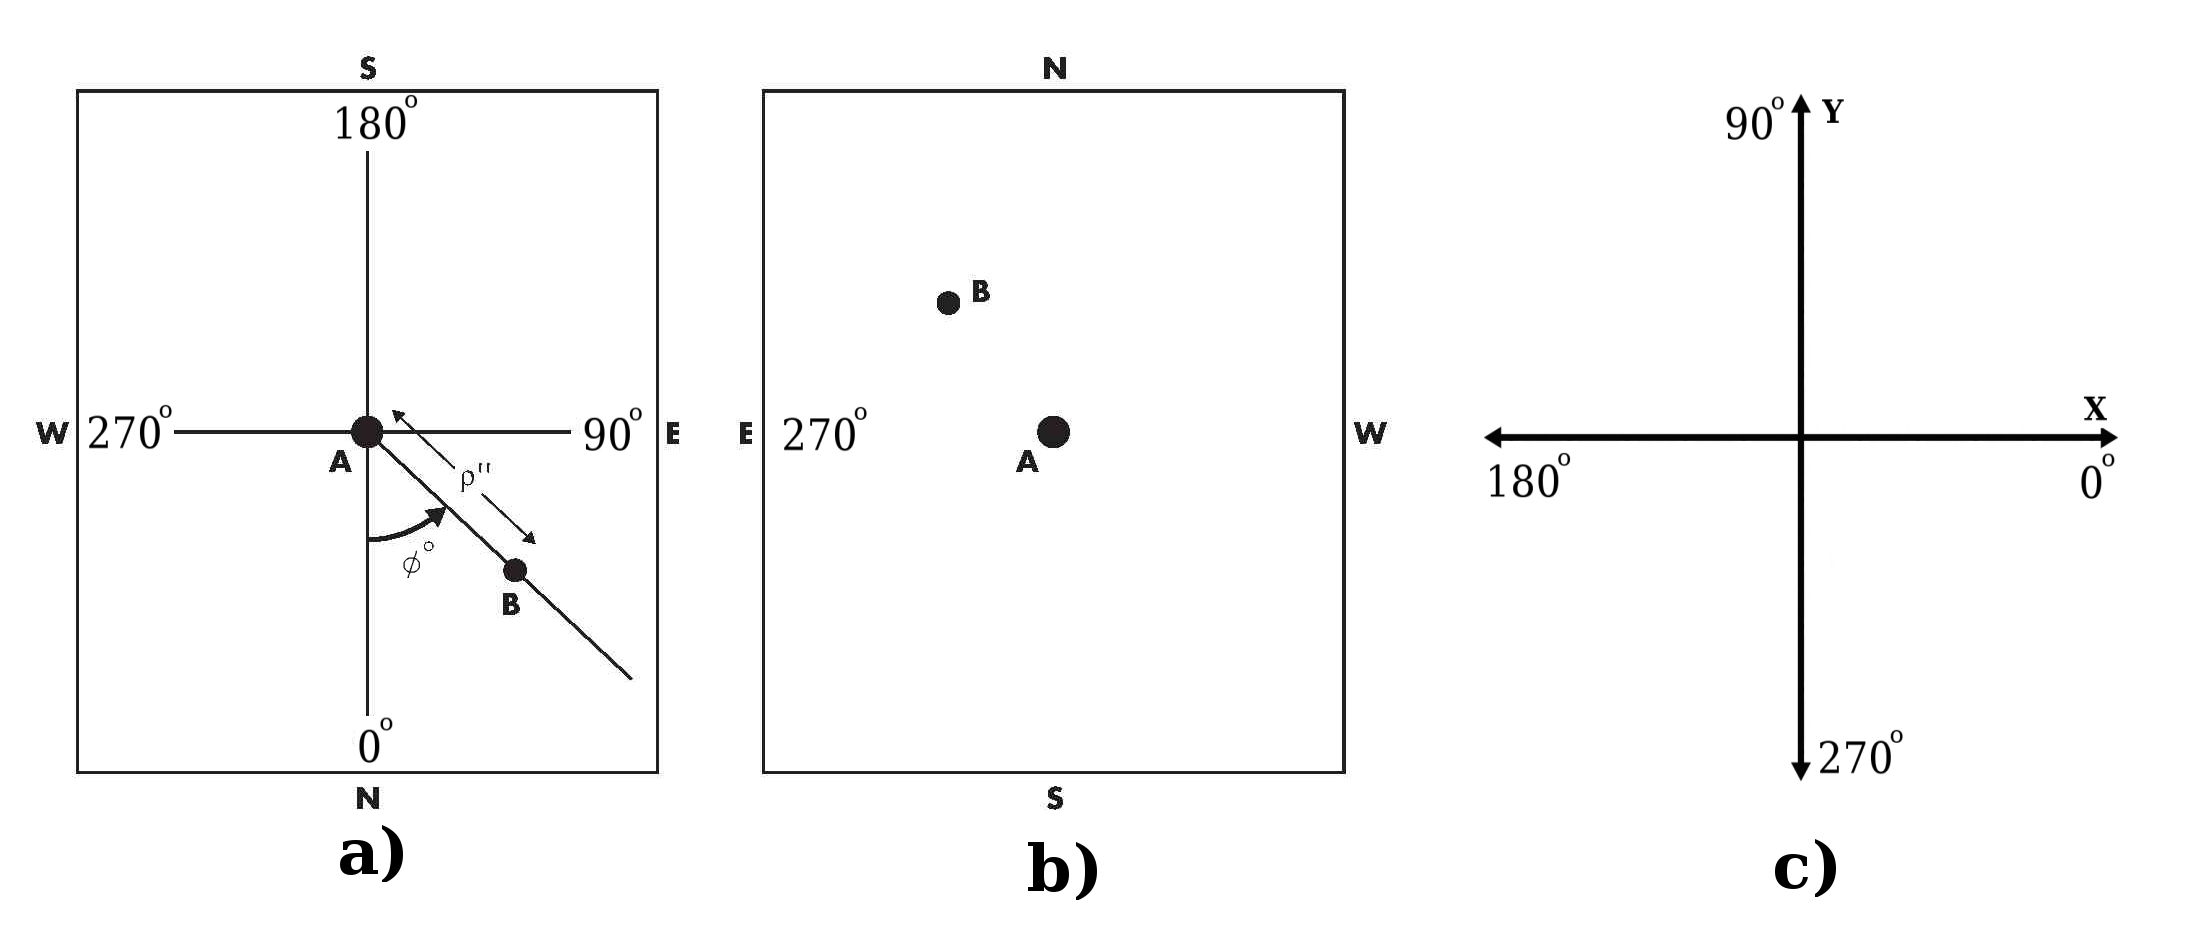
\includegraphics[scale=0.9]{Argyle-oribit-plots1-cropped-AND-cartesianCoordsPlot.jpg}
\caption[View of a Binary System]{ View of a binary system through a) A telescope, and b) The naked eye, both compared to c) 2D Cartesian coordinate system. \citet{Argyle}. }
\label{fig:4}
\end{center}
\end{figure}

%\begin{figure}[ht]
%	\begin{minipage}{0.45\hsize} %left picture
 %   \begin{center}
 %   \includegraphics[scale=0.7]{Figures/Argyle-oribit-plots1-cropped.jpg}
 %   \end{center}
 %   \caption[View of a Binary System]{ View of a binary system through a. A telescope, and b. The naked eye, %			\citet{Argyle}. }
%    \label{fig:4}
%  \end{minipage}
%  \begin{minipage}{0.4\hsize} %right picture
%    \begin{center}
%    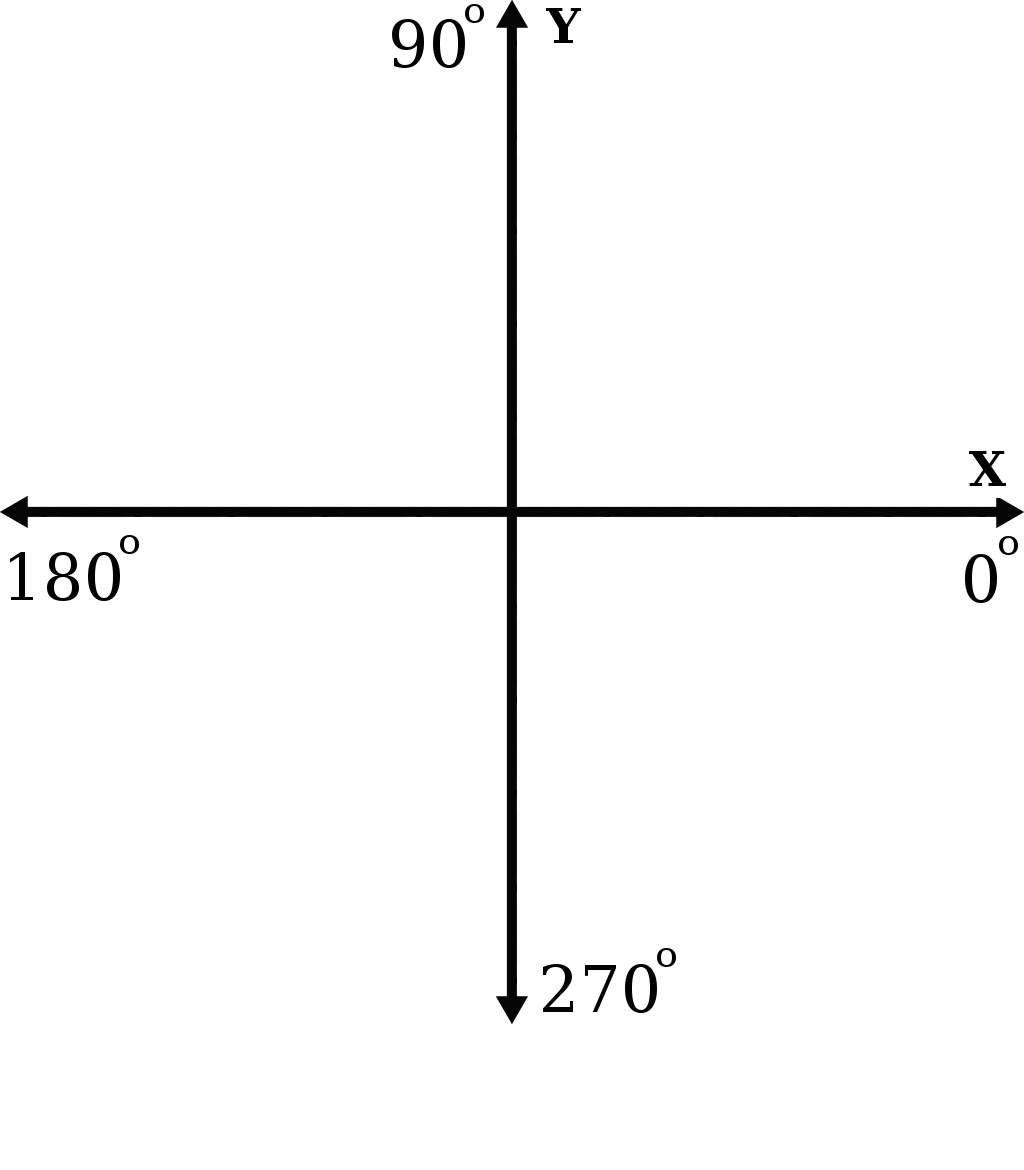
\includegraphics[scale=0.18]{Figures/CartesianCoordSystem-mine2.jpeg}
%    \end{center}
 %   \caption{2D Cartesian coordinate system.}
%    \label{fig:4.5}
%  \end{minipage}  
%\end{figure}


\begin{figure}[ht]
\begin{center}
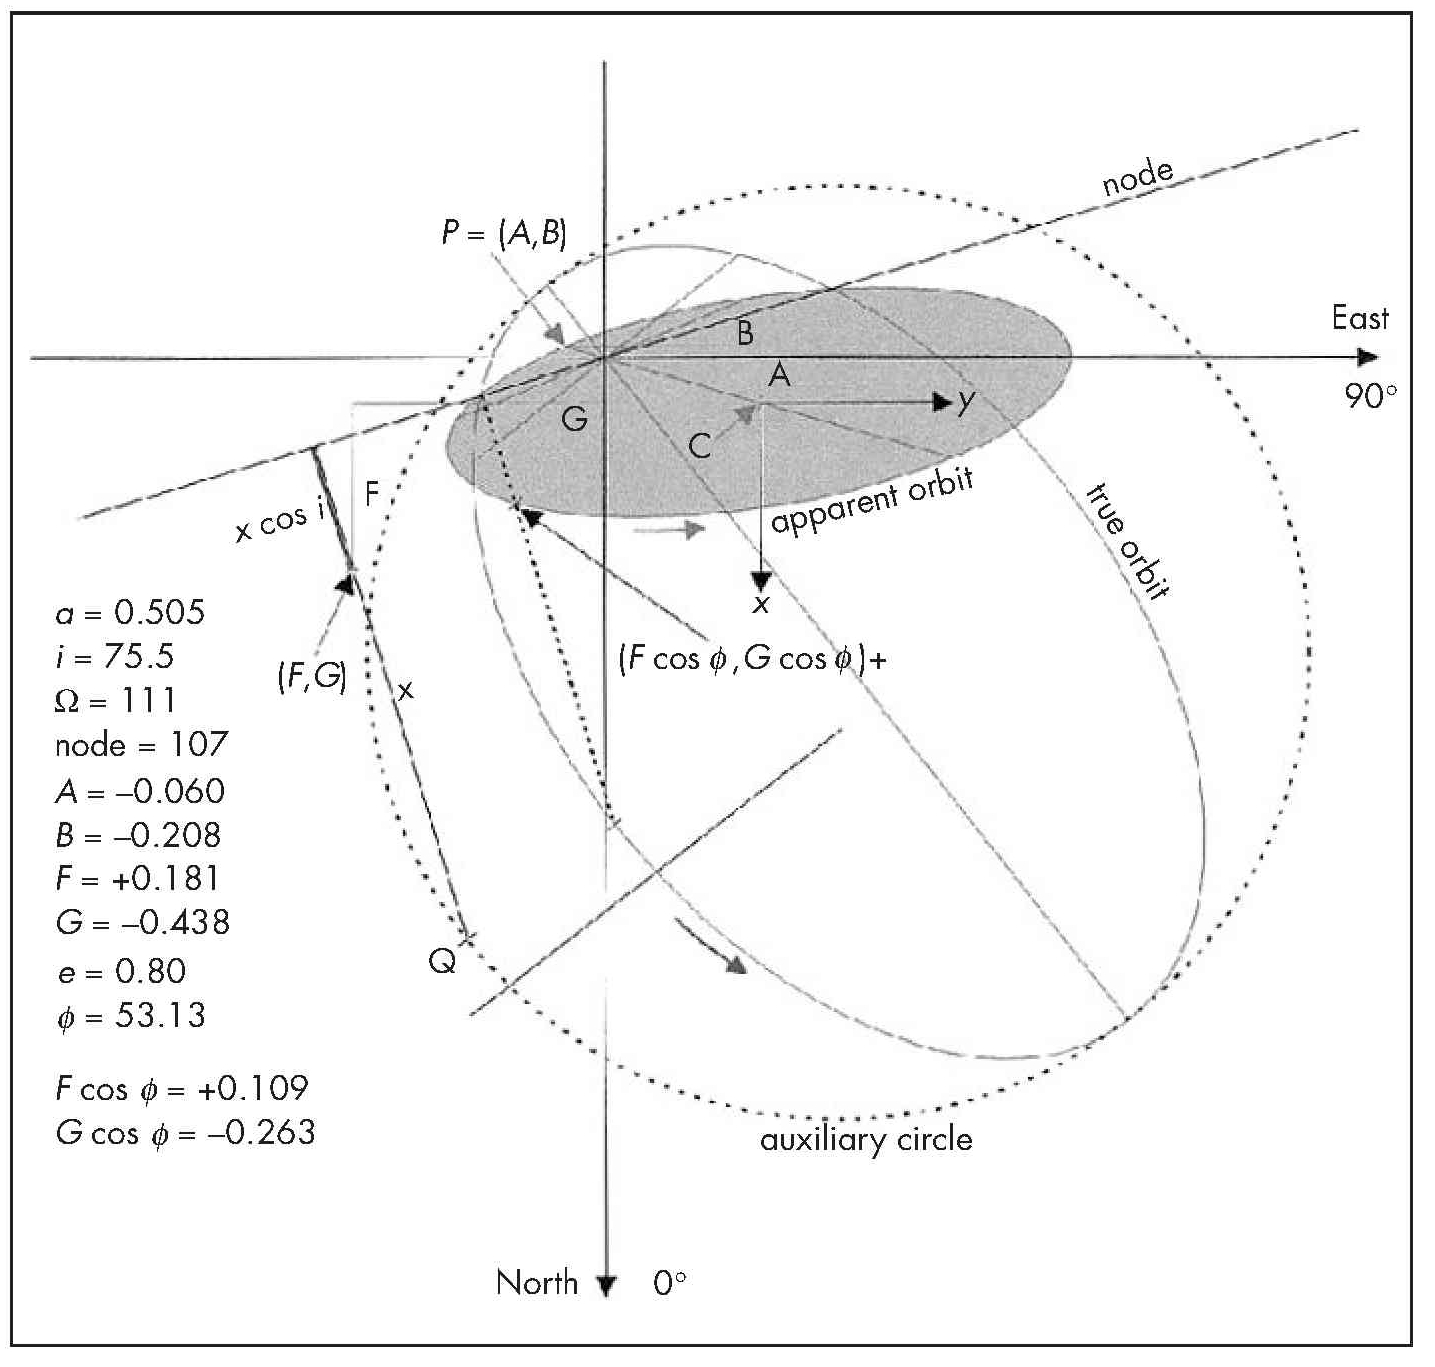
\includegraphics[scale=0.9]{Argyle-oribit-plots2-cropped.jpg}
\caption[Apparent and True orbital ellipses]{ Plot of apparent and true orbital ellipses, and the Thiele-Innes elements, \citet{Argyle}. }
\label{fig:apparentTrueEllipses}
\end{center}
\end{figure}

In the case where the data is measured as the difference in Right Ascension ($\alpha$) and Declination ($\delta$) of the companion from the primary star, in units of [$\arcsec$], these match the E=y and N=x respectively.  This allows for direct comparison of the data to the values calculated in equations  (\ref{eq:28-1a}) and (\ref{eq:28-1b}).  If these units need to be converted to $\phi$ and $\rho$, then the following conversions can be used.

\begin{subequations}
\begin{align}\label{eq:RADECtoPA}
\phi =&   \tan^{-1}\bigg(\frac{\alpha}{\delta} \bigg)\\
\label{eq:RADECtoSA}
\rho =&   \sqrt{\delta^2+\alpha^2}
\end{align}
\end{subequations}

The conditionals below are needed to correct the resulting angle from (\ref{eq:RADECtoPA}) for all four quadrants.

\begin{equation}\label{eq:4.1.PAcorrection}
\phi_{corrected} = \left\{ \begin{array}{l l l} \phi& \quad \text{ if in quadrant 1}\\ \phi + \pi& \quad \text{ if in quadrant 2 or 3}\\ \phi + 2\pi& \quad \text{ if in quadrant 4}  \end{array} \right.
\end{equation}

\begin{subequations}
\begin{align}\label{eq:RADECtoPAerr}
\Delta\phi =&   \frac{\bigg(\frac{\alpha}{\delta}\bigg) \sqrt{\bigg( \frac{\Delta\alpha}{\alpha} \bigg)^2 \bigg( \frac{\Delta\delta}{\delta} \bigg)^2} }{1.0+\bigg(\frac{\alpha}{\delta} \bigg)^2}\\
\label{eq:RADECtoSAerr}
\Delta\rho =&   \rho\Bigg(\frac{\alpha\Delta\alpha + \delta\Delta\delta}{\alpha^2 + \delta^2} \Bigg)
\end{align}
\end{subequations}

Noting that the $\delta$ and $\alpha$ here represent a difference in the values between the primary and companion instead of the more commonly used values of just the Right Ascension and Declination of each object.  This was chosen here to make it easier to express the values in the error calculations of equations (\ref{eq:RADECtoPAerr}) and (\ref{eq:RADECtoSAerr}).

%-----------------------------------------
\clearpage
\subsubsection{Thiele-Innes ``Shortcut" Approach}\label{sec:TH_I_shortcut}

This is the approach implemented in the C++ code used during the simulation as it is the fastest.

That described in section \ref{sec:TH_I} is the general description of the method to use the Thiele-Innes Constants to solve for the orbital parameters of a binary system.  Due to the inputs to this method being those constants, equations (\ref{eq:25a} - \ref{eq:28}) must be used to solve for the orbital parameters from them.  This is a little cumbersome and can be simplified.

The way to do this would be to still use equations (\ref{eq:24a} - \ref{eq:24d}), and (\ref{eq:28} - \ref{eq:28-3b}), but accept the orbital parameters needed to solve for the Thiele-Innes Constants in those equations as inputs.  Then, the same equations would be used for a comparison of the x and y values predicted to those measured.  While this may seem to be a trivial difference of the inputs to the calculations, it has some major benefits.

The first benefit is that the simulator which utilizes this model can perform is own controls on the limits of the orbital parameter's ranges being explored.  By looking at equations (\ref{eq:25a} - \ref{eq:27}) one can see they are comprised of various combinations of the orbital elements.  This makes it nearly impossible to directly impose strict limits to their allowed values, and values outside of the ranges desire could be sampled.  Restricting the parameter space is an important approach to help the simulator avoid getting caught in local minima.

A second benefit is the ability to take advantage of priors when choosing the values for the orbital parameters.  The theory behind priors and the role they play in Bayesian Inference problems was discussed in section 3.1 of my MSc thesis (available upon request).  In short, the choice of a prior, and its corresponding distribution that samples are drawn from, can make large changes on the posterior probability distribution produced.  Any knowledge of trends or physically justified characteristics of the parameters can be taken into account through the priors.  Without the ability to include this information, the resulting posterior can be skewed, or inaccurate.

Therefore, this modification, or shortcut, to the original Thiele-Innes method solves these problems.

\clearpage

\pagebreak
%----------------------------------------------------------------------------------------------------------------------------------

\subsection{Radial Velocity Model}\label{sec:RV-OrbModels}

In the case of calculating the radial velocity residuals, there are various forms of the equation to calculate predicted radial velocity of the host star due to its companion's motion.

One very important thing that needs to be taken into account for radial velocity equations, that does not effect in direct imaging calculations, phase offset.  This is the phase difference between the location of the companion at closest approach and inferior conjunction; in cases where the inclination is $\sim$90, the companion passes in front of the primary and the inferior conjunction is also referred to as the location of center transit.  To take this into account, a manipulated version of the Mean Anomaly equation is used, which in turn effects the value of the True Anomaly used in the following radial velocity calculations.
%\subsubsection{Inputs}
\begin{table}[h]
\centering
\caption{ Inputs to the Radial Velocity Model.}
\begin{tabular}{c c c}
\hline\hline
Parameter & Description & Typical Range \\
\hline
t* & epoch of observation/image [julian date] & n/a\\
Sys$\_$Dist* & measured system distance from Earth [PC] &  [0.01,50.0]\\
{\it i} & inclination [$^{\circ}$] & [0,180]\\
$\omega$ & Argument of Periapsis [$^{\circ}$] & [0,360]\\
e & eccentricity of orbits [unitless] & [0.001,0.999]\\
T & Last Periapsis Epoch/time [julian date] & [t-period,t]\\
$T_c$* & Last Transit Center Epoch/time [julian date] & [t-period,t]\\
period & period of orbits [yrs] & [1.0,100.0]\\
a*** & Total Semi-major axis [AU]  & [0.1,200] \\
Mass1*** & Mass of primary star [M$_{\sun}$] & [0.001,10] \\
Mass2*** & Mass of companion [M$_{\sun}$] & [0.001, Mass1] \\
K*** & Semi-major Amplitude of primary star [m/s]& [1,500]\\
verbose & Send prints to screen? [True/False](Default = False) & n/a\\
\hline
\end{tabular}
\\
  * = Normally measured/known (ie. not random numbers).\\
 *** = Optional.
\end{table}

%\subsubsection{Outputs}

\begin{table}[h]
\centering
\caption{ Outputs of the Radial Velocity Model.}
\begin{tabular}{c c}
\hline\hline
Parameter & Description \\
\hline
vr & Radial Velocity of primary due to companion [m/s] \\
K & Semi-major Amplitude of primary star [m/s]\\
\hline
\end{tabular}
\end{table}

\pagebreak

Use the Mean Motion, n, time of current epoch (t), time of last periapsis (T), and time of transit center transit (Tc) to get the updated Mean Anomaly:
\begin{subequations}\label{eq:RV-Ma}
\begin{align}
phase& = \frac{Tc-T}{period_{days}} \\
%int\bigg(\frac{Tc-T}{period_{days}}\bigg)period_{days}
\label{eq:RV-Mb}
M& = n \bigg[ \frac{(t-T)}{365.25} +phase \bigg]\\
\end{align}
\end{subequations}
%where `int()' refers to taking the integer value of what is in the brackets.  
The phase of the companion in Equation (\ref{eq:RV-Ma}) is unit-less value between 0 and 1.  In Equation (\ref{eq:RV-Mb}), the first term is essentially a fraction of how far the current epoch is away from the time of last periapsis multiplied by the Mean Motion throughout the orbit, resulting in units of radians.  Following these equations (\ref{eq:4.1.3})-(\ref{eq:4.1.5b}) would be used to calculate the True Anomaly needed in the radial velocity calculations shown below.  This modified version of the Mean Anomaly equation is only needed when the eccentricity is non-zero, else Tc is set equal to {\it T} resulting in a zero phase, so this version reduces to the original form shown in (\ref{eq:4.1.2}).
%It was found that because of the sine function in (\ref{eq:4.1.4}), shifting the phase ahead into a positive value within $2\pi$ was the best .

The most common form of the radial velocity equation is:
\begin{equation}\label{eq:rvStandard}
vr =  K[\cos(\theta+\omega_2)+e \cos(\omega_2)]
\end{equation}
where {\it K} is the semi-major amplitude of the radial velocity curve, as can be seen in Figure \ref{fig:RVplot}.

The different formulations for calculating {\it K} are related to each other by Kepler's third law, given in Equation (\ref{eq:28}).

To find the radial velocity of the primary star due to companion's orbital motion: %(version used in VRcalcStarStar:VRcalculator):
\begin{equation}\label{eq:30}
K_s = \bigg[\frac{2\pi G}{P}\bigg]^{1/3}\frac{M_2}{(M_1+M_2)^{2/3}}\frac{\sin(i)}{\sqrt{1-e^2}} = \frac{2\pi a_1\sin(i)}{P\sqrt{1-e^2}}
\end{equation}

When the companion is a planet, it can commonly be assumed that Mass$_{planet} \ll$ Mass$_{star}$, so $M_1+M_2 \approx M_1$.  This simplifies the equation for {\it K} to:
\begin{equation}\label{eq:31}
K_s = \bigg[\frac{2\pi G}{P}\bigg]^{1/3}\frac{M_2}{M_1^{2/3}}\frac{\sin(i)}{\sqrt{1-e^2}}
\end{equation}

As the mass of each object is needed to calculate the semi-major axis of the primary, a$_1$, using the second form in (\ref{eq:30}) keeps things simple.

%Velocity residual due to planet around primary star (version used in VRcalcStarPlanet: VRcalculatorsemi-majorType):
%\begin{equation}\label{eq:29}
%vr_p = \frac{2\pi a_1\sin(i)}{P\sqrt{1-e^2}}[\cos(\theta+\omega)+e \cos(\omega)]= K_p[\cos(\theta+\omega)+e \cos%(\omega)]
%\end{equation}

%Velocity residual due to planet around primary star (version used in VRcalcStarPlanet:VRcalculator):
%\begin{equation}\label{eq:31}
%vr_p = \bigg[\frac{2\pi G}{P}\bigg]^{1/3}\frac{M_2\sin(i)}{M_1^{2/3}}\frac{1}{\sqrt{1-e^2}}[\cos(\theta+\omega)+e \cos(\omega)] = K_p[\cos(\theta+\omega)+e \cos(\omega)]
%\end{equation}

In \citet{Shulze-Hartung} an alternative formulation for the radial velocity equation is used that inputs the Eccentric Anomaly, E, instead of the True Anomaly, $\theta$.  The difference between these is is just a choice of parameters and they are both mathematically equivalent.

Velocity residual due to companion star, or planet, used in \citet{Shulze-Hartung}:
\begin{equation}\label{eq:32}
vr = \frac{2\pi a_1 \sin(i)}{P(1-e\cos(E))}[\sin(E)\sin(\omega)-\sqrt{1-e^2}\cos(E)\cos(\omega)]
\end{equation}

%\begin{subequations}\label{eq:32.2}
%\begin{align}
%vr_p& = \frac{2\pi a_1 \sin(i)}{P}\bigg [\frac{\sin(E)\sin(\omega)-\sqrt{1-e^2}\cos(E)\cos(\omega)}{(1-e\cos(E))}\bigg]\\
%& =\bigg[ \frac{2\pi G}{P}\bigg]^{1/3} \bigg[\frac{M_p \sin(i)}{(M_p+M_1)^{2/3}} \bigg] \bigg [\frac{\sin(E)\sin(\omega)-\sqrt{1-e^2}\cos(E)\cos(\omega)}{(1-e\cos(E))}\bigg]
%\end{align}
%\end{subequations}

Although, whether $\omega$ is equal to $\omega_1$ or $\omega_2$ is not properly described in the paper.  Through personal communications with the author, it was clarified to be $\omega_2$ in all cases.  %Following their convention, we set $\omega_1 = \omega_2+\pi$, as it is arbitrary as long as it the convention is mentioned in any resulting research papers.

Finally the ${\chi}^{2} $ is calculated following:
\begin{equation}\label{eq:33}
{\chi}^{2} \equiv  \sum_{i=1}^{i=E} \frac{(model_i - observed_i)^{2}}{\sigma^{2}_i} = \sum_{i=1}^{i=E} \frac{[(vr_c+vr_p) - (RV_{data}-\gamma)]^{2}}{\sigma^{2}_i}
\end{equation}

where $\gamma $ is the velocity offset of that instrument.  In the case that the velocity of the system's center of mass WRT the Earth has not been removed, the observed component in (\ref{eq:33}) becomes ($RV_{data}-\gamma_{Instrument}-\gamma_{COM}$) (\citet{Paddock} \& \citet{Shulze-Hartung}).

%----------------------------------------------------------------------------------------------------

\pagebreak
\bibliography{SMODT-citations}
\clearpage

\end{document}









